\paragraph{Two-strains Tuberculosis Model.}
Seeking to reduce the latent and infectious groups with the 
resistant-strain tuberculosis, in \cite{Lenhart2002} the authors  use 
controls ro represents 	two types of treatments in a tuberculosis model 
which consider the effect of treatment in two kinds of strains. The 
controlled version reads:
%
%	
%	\begin{equation}\label{eqn:two_strain_TB}
%	  \begin{aligned}
%	    \frac{dS}{dt} &=
%		    \Lambda - \beta_1 S \frac{I_1}{N} 
%		    - \beta^{*} S \frac{I_2}{N}
%		    - \mu S
%		  \\
%		  \frac{L_1}{dt} &=
%			  \beta_1 S \frac{I_1}{N}
%			  - (\mu + k_1) L_1
%			  +  p r_2 I_1
%				+ \beta_2 T \frac{I_1}{N}
%				- \beta^{*} L_1 \frac{I_2}{N}
%			\\
%			\frac{I_1}{dt} &= 
%				k_1 L_1
%				- (\mu + d_1) I_1
%				-r_2 I_1
%			\\
%			\frac{L_2}{dt} &=
%				q r_2 I_1
%				- (\mu + k_2) L_2
%				+ \beta^{*} (S + L_1 + T) \frac{I_2}{N}
%			\\
%			\frac{I_2}{dt} &=
%				k_2 L_2 - (\mu + d_2) I_2
%			\\
%			\frac{d T}{dt} &=
%				r_1 L_1
%				+ (1 - (p + q)) r_2 I_1
%				- \beta T \frac{I_1}{N}
%				- \beta^{*} T \frac{I_2}{N}
%				-\mu T ~.
%	  \end{aligned}
%	\end{equation}
%
%
	\begin{equation}\label{eqn:TB}
	  \begin{aligned}
	    \frac{dS}{dt} &=
		    \Lambda - \beta_1 S \frac{I_1}{N} 
		    - \beta^{*} S \frac{I_2}{N}
		    \mu S
		  \\
		  \frac{L_1}{dt} &=
			  \beta_1 S \frac{I_1}{N}
			  - (\mu + k_1) L_1
			  - u_1 (t) r_1 L_1
			  + (1 - u_2 (t)) p r_2 I_1
				+ \beta_2 T \frac{I_1}{N}
				- \beta^{*} L_1 \frac{I_2}{N}
			\\
			\frac{I_1}{dt} &= 
				k_1 L_1
				- (\mu + d_1) I_1
				-r_2 I_1
			\\
			\frac{L_2}{dt} &=
				(1 - u_2(t)) q r_2 I_1
				- (\mu + k_2) L_2
				+ \beta^{*} (S + L_1 + T) \frac{I_2}{N}
			\\
			\frac{I_2}{dt} &=
				k_2 L_2 - (\mu + d_2) I_2
			\\
			\frac{d T}{dt} &=
				u_1(t) r_1 L_1
				+ (1 - (1 - u_2(t))(p + q)) r_2 I_1
				- \beta T \frac{I_1}{N}
				- \beta^{*} T \frac{I_2}{N}
				-\mu T.
	  \end{aligned}
	\end{equation}

	\citeauthor*{Lenhart2002} consider time dependent 
optimal control strategies associated with \emph{case holding} and 
\emph{case finding}. They 
incorporates the case finding control by adding a term which identifies and 
cure a fraction o latent individuals. Case finding consequently reduces the 
rate of disease development by latent individuals. The authors includes case 
holding by adding a term which may decrease the treatment failure rate of 
individuals with sensitive  TB, so, this control reduce the incidence of drug 
resistant TB. In model \eqref{eqn:TB}, $u_1$ denotes the fraction of 
typical TB latent individuals that is identified and will put under 
treatment \textemdash case finding control \textemdash and $1 - u_2$ represents 
the effort that prevents the failure treatment in typical TB infectious 
individuals.

	The controls $u_1$ ,$u_2$ reduce the latent and infected 
groups with resistant TB. However, the case holding and the case finding 
strategies produces a economic fee. In \cite{Lenhart2002} the authors use
\begin{equation}
	 J(u_1, u_2) =
		 \int_0 ^ {t_f}
			 \left[
				 L_2(t) + I_2(t) 
				 + \frac{B_1}{2} [u_1(t)] ^ 2
				 + \frac{B_2}{2} [u_2(t)] ^ 2
			 \right]dt,
\end{equation}
to describe the regarding cost.
\begin{table}
	\begin{center}
		\begin{tabular}{@{}rll@{}} 
			$S:$
			&
				Susceptible
			\\
			$I:$ 
			&	Infected
			\\
			$R:$ 
			&	Recover
			\\
			\\
			%\toprule
			\multicolumn{1}{c}{Parameter}
			&
			\multicolumn{1}{c}{Meaning}
			& 
			\multicolumn{1}{c}{Value}
			\\
				\midrule
				$\beta$
				& 
					Transmission probability
				&
					---
			\\
				$\gamma$
				&
					Recover rate
			\\
				$\mu$
				&
					Natural death rate
			\\
				$K$
				&
					Carrying capacity
			\\
			\bottomrule
		\end{tabular}
		\caption{Variables and parameters description}
	\end{center}
\end{table}

In figure [] we show the effect of case finding and case holding controls.

\begin{figure}
  \centering
  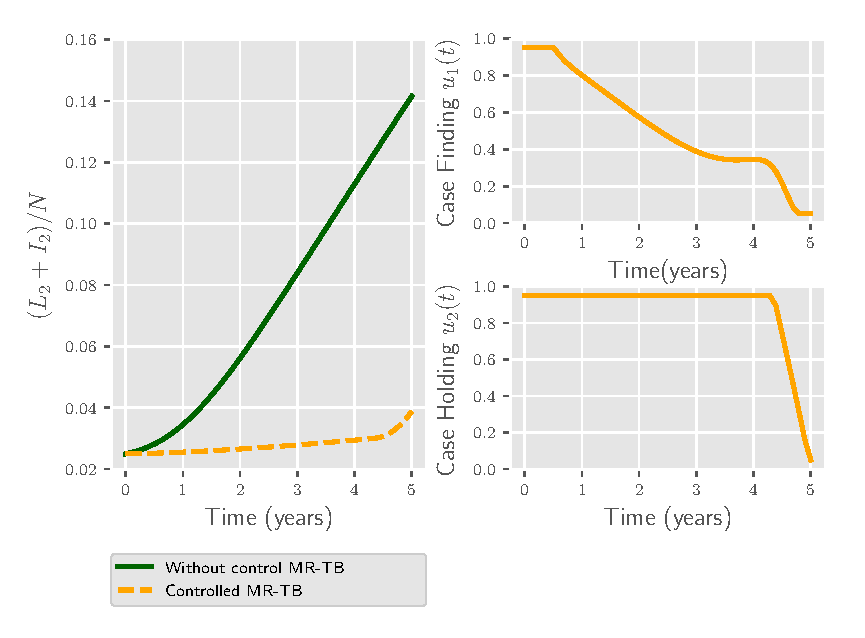
\includegraphics[width=0.7\linewidth]{Figures/figure_1_two_strain_tbm}
  \caption{Normalized infected population according to the parameters in 
  table [*]. Here the green line represents the infected population whitout 
  control. As we see, case finding $u_1(t)$ and case holding $u_2(t)$, 
  dramatically diminish the density of infected with multiresistan TB.}
  \label{fig:figure1twostraintbm}
\end{figure}


In figure [] we show the effect of the parameter $\beta_3$. As wee see the 
simulation suggest that...

\begin{figure}
  \centering
  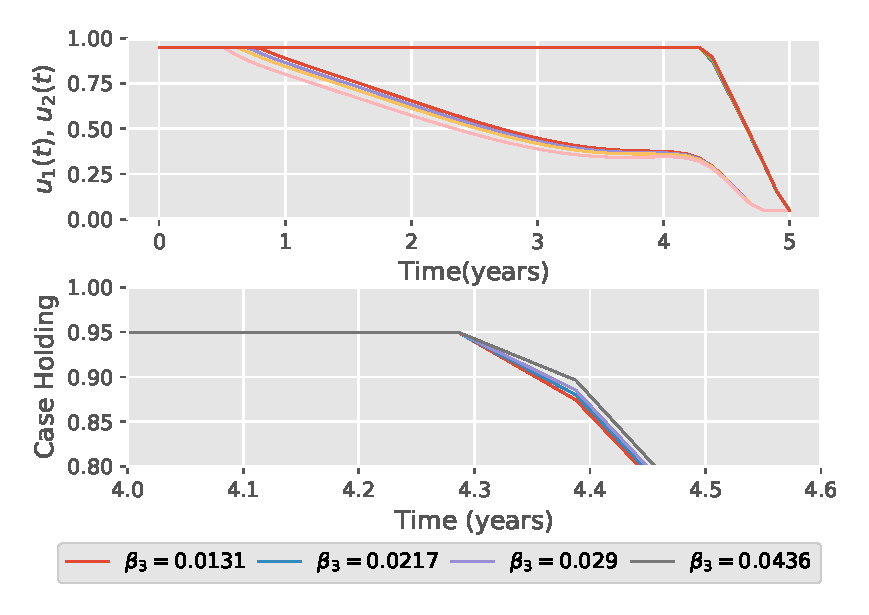
\includegraphics[width=0.7\linewidth]{Figures/figure_2_two_strain_tbm}
  \caption{}
  \label{fig:figure2twostraintbm}
\end{figure}


